\documentclass[crop,tikz,10pt]{standalone}

\usepackage{tikz-qtree}
\usetikzlibrary{positioning}

\definecolor{bg1}{RGB}{244,231,195}
\definecolor{bg2}{RGB}{234,204,161}
\definecolor{l1}{RGB}{209,148,106}

\begin{document}

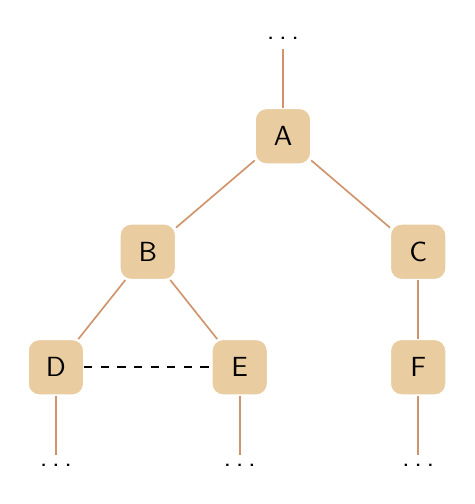
\begin{tikzpicture}[
    font=\sffamily,
    l/.style={
        line width=0.6pt,
        color=l1
    },
    e/.style={
        rounded corners, minimum size=2em,
        fill=bg2, draw=white, line width=0.4pt
    },
    d/.style={dashed, line width=0.8pt}
]

\node [e] (A) {A};
\node [e,below left =0.75cm and 1cm of A] (B) {B};
\node [e,below right=0.75cm and 1cm of A] (C) {C};
\node [e,below left =0.75cm and 0.45cm of B] (D) {D};
\node [e,below right=0.75cm and 0.45cm of B] (E) {E};
\node [e,below=0.75cm of C] (F) {F};

\draw (A) edge [l] (B);
\draw (A) edge [l] (C);
\draw (B) edge [l] (D);
\draw (B) edge [l] (E);
\draw (C) edge [l] (F);

\node [above=0.75cm of A] (root) {\ldots\unkern};
\node [below=0.75cm of D] (d_) {\ldots\unkern};
\node [below=0.75cm of E] (e_) {\ldots\unkern};
\node [below=0.75cm of F] (f_) {\ldots\unkern};

\draw (A) edge [l] (root);
\draw (D) edge [l] (d_);
\draw (E) edge [l] (e_);
\draw (F) edge [l] (f_);

\draw [d] (D) edge (E);

\end{tikzpicture}
\end{document}
